%% This is file AJCEAM-paper.tex is the template file for publications
%% in the "
%% from Universidade Federal do Tocatins, Brazil,
%% https://sistemas.uft.edu.br/periodicos/index.php/AJCEAM/index
%% This file was originally written by Tiago Almeida.
%% First revision: 2019-10-29
%% Second revision:
%%
%% History:
%%           2019-10-29 - First version by Tiago Almeida <tiagoalmeida@uft.edu.br>.
%%           2020-04-09 - English revision by Caio Machado <caio.machado@uft.edu.br>
%%

% Options
%     eng:   English Language
%     por:   Portuguese Language
%     blind: The version for reviewers is compiled (author data is hidden)

\documentclass[eng]{ajceam-class}

% Publication Title
\title{Detección multietiqueta de anomalías en resonancias magnéticas de rodilla mediante aprendizaje profundo}

\usepackage{tabularx}

% Short title for the header (copy the main title if it is not too long)
\shorttitle{Detección de anomalías en resonancias de rodilla}
       
% Authors
\author[1]{Jenaro Alcaraz Sargosa (A0164685)}
\author[2]{Hector Fernando Piñon Soto (A01564220)}
\author[3]{Javier Sebastien Zagal Rodriguez (A01752711)}

% Author Affiliations
\affil[1]{Instituto Tecnológico de Estudios Superiores de Monterrey (ITESM), Departamento de Ingeniería y Ciencias, Nuevo Leon, México}


% Surname of the first author of the manuscript
\firstauthor{Alcaraz Sargosa, Piñon Soto y Zagal Rodriguez}

%Contact Author Information
\contactauthor{Jenaro Alcaraz Sargosa}           % Name and surname of the contact author
\email{Por confirmar}            % Contact Author Email

% Publication data (will be defined in the edition)
\thisvolume{01}
\thisnumber{01}
\thismonth{Octubre}
\thisyear{2026}
\publicationdate{12/10/2026}

% Place your particular definitions here
\newcommand{\vect}[1]{\mathbf{#1}}  % vectors

% Insert here the abstract in English language
\abstract{
Este proyecto propone desarrollar un modelo de aprendizaje profundo que estime la presencia de anomalías en estudios de resonancia magnética de rodilla, utilizando el conjunto RSNA Knee Abnormality Detection de Kaggle. Se plantea una clasificación multietiqueta, en la cual un estudio puede presentar varios hallazgos simultáneamente. Se compararán una CNN de referencia y una arquitectura preentrenada adaptada al análisis de múltiples cortes. El objetivo es evaluar su capacidad predictiva y su costo computacional como prototipo de investigación, con posibles aplicaciones futuras de apoyo a la revisión radiológica. Este tercer avance incorpora un primer entrenamiento con una red completamente conectada, antes de aplicar las arquitecturas convolucionales propuestas. Se utilizaron 58 estudios con etiquetas explícitas, separados en 46 para entrenamiento y 12 para validación, y se probaron tres configuraciones durante 40 épocas. Las curvas muestran sobreajuste en los tres casos. La menor pérdida de validación entre las redes fue 0.6104, mientras que una referencia constante obtuvo 0.5850. Estos resultados permiten documentar el funcionamiento del entrenamiento y sus limitaciones como un primer experimento.
}

% Insert here the keywords of your work in English language
\keywords{
Redes neuronales convolucionales, resonancia magnética, rodilla, clasificación multietiqueta, aprendizaje por transferencia.
}

\begin{document}


\maketitle
\thispagestyle{fancy}


\section{Introducción}

El proyecto aborda la clasificación automática de imágenes médicas mediante redes neuronales convolucionales (CNN). Nuestro equipo eligió trabajar con resonancias de rodilla para conectar el aprendizaje de estas arquitecturas con una tarea concreta y participar en una competencia de investigación en la plataforma de \textit{Kaggle}. En la primera entrega se definió el alcance de construir y evaluar una red que procese un estudio y produzca probabilidades de presenciar ciertos síntomas o anormalidad en una resonancia.

es importante mencionar que la salida del modelo no será un diagnóstico clínico definitivo o universal. El interés es poder establecer un procedimiento reproducible de preparación de datos, entrenamiento y evaluación de la red que pueda desarrollarse en los proximos avances.

En este tercer avance comenzamos con una red completamente conectada, también conocida como \textit{feedforward}. La intención es correr un primer entrenamiento real y observar qué sucede al cambiar algunos hiperparámetros. Las CNN que ya propusimos quedan para el siguiente avance. Por ahora nos interesa comprobar que podemos preparar las imágenes, entrenar una red y explicar sus curvas, aunque los resultados de evaluación sean bajos.

\section{Contexto del problema}

La resonancia magnética permite estudiar estructuras de la rodilla relevantes para la evaluación de lesiones. Sin embargo, interpretar un examen exige revisar numerosas imágenes y relacionar información de diferentes vistas. Constantemente se dice que esta interpretación consume tiempo y puede presentar variabilidad, por lo que se intenta aplicar el uso de aprendizaje profundo como apoyo a especialistas \cite{bien2018}.

Nos interesa este problema porque combina una necesidad real con un reto de aprendizaje. Debemos de identificar patrones visuales sutiles y reunir evidencia distribuida entre cortes. Una anomalía puede presentarse junto con otras asi que asignar una sola categoría a cada estudio sería deficiene. La solución propuesta debe estimar cada hallazgo por separado.

El desarrollo de una red podría contribuir a priorizar estudios para revisión y organizar colecciones de imágenes para investigación, aunque es cierto que los resultados deberian de considerarsecomo una segunda lectura en casos reales. Estas son aplicaciones potenciales pero beneficios demostrados por nuestro proyecto. Como antecedente real, MRNet fue evaluado para reconocer anomalías y lesiones de ligamento y menisco. Pero el estudio va más allá porque también se usó para profundizar en el efecto de sus predicciones sobre la interpretación de expertos \cite{bien2018}.

El valor tecnico que obtenemos nosotros consiste en aprender a construir una CNN y evaluar sus errores bajo condiciones más complejas que las de un conjunto de imágenes convencional (como el dataset de moda). También interesa analizar qué sucede cuando un modelo se enfrenta a estudios de distintos equipos e instituciones. Una puntuación alta en un conjunto de datos interna no garantiza que el sistema funcione igual en otro entorno.

Nuestro desarrollo de una red es meramente con propósito de investigación. La licencia MIRA (que posee el dataset de la competencia) restringe el uso de datos y los fines autorizados y excluye su empleo en diagnóstico o atención de pacientes \cite{mira}. El alcance de esta entrega es metodológico y experimental, ya que al final del dia es para una Unidad de Formación.

\section{Descripción del conjunto de datos}

\subsection{Origen, tamaño y organización}

Se utilizará RSNA Knee Abnormality Detection, organizado por la Radiological Society of North America y alojado en Kaggle. La ficha publica 819\,640 archivos y 569.76 GB. Incluye estudios internacionales, series DICOM y archivos CSV; cada imagen DICOM corresponde a un corte. Hay aproximadamente 1\,300 estudios de prueba \cite{rsnadata}.

Las cantidades no equivalen a ejemplos independientes de entrenamiento. Al inspeccionar \texttt{train.csv} confirmamos 4\,407 estudios de entrenamiento: 58 tienen las doce etiquetas binarias y 4\,349 cuentan con reportes sin esas etiquetas. Para el primer experimento de esta entrega utilizamos únicamente los 58 estudios etiquetados.

\subsection{Categorías y etiquetas}

Los doce hallazgos son:
\begin{itemize}
    \item Lesión del ligamento cruzado anterior.
    \item Lesión del ligamento colateral medial.
    \item Rotura del menisco medial.
    \item Rotura del menisco lateral.
    \item Osteoartritis tibiofemoral medial.
    \item Osteoartritis tibiofemoral lateral.
    \item Osteoartritis patelofemoral.
    \item Derrame articular.
    \item Sinovitis.
    \item Quiste de Baker.
    \item Contusión ósea.
    \item Fractura.
\end{itemize}

 Solo un subconjunto de entrenamiento (58) posee etiquetas explícitas. El resto (4\,349) disponen de reportes radiológicos. Estos reportes no estarán disponibles en prueba \cite{rsnadata}.

\subsection{Ejemplos y consideraciones}

Las imágenes incluyen distintos cortes (sagitales, coronales y axiales), una serie suele tener 20--45 cortes (varios fotogramas o imágenes de diferentes capas de la rodilla) y un estudio entero de una sola rodilla se puede conformar por una o mas series (ejemplo explícito de un corte en la Fig.~\ref{fig:corte-rodilla}). Varían en intensidad, orientación y resolución \cite{rsnadata}. Como ejemplos conceptuales de clasificación, un estudio podría presentar lesión ligamentaria y derrame al mismo tiempo, o quizas carecer de los doce padecimientos.

\begin{figure}[H]
    \centering
    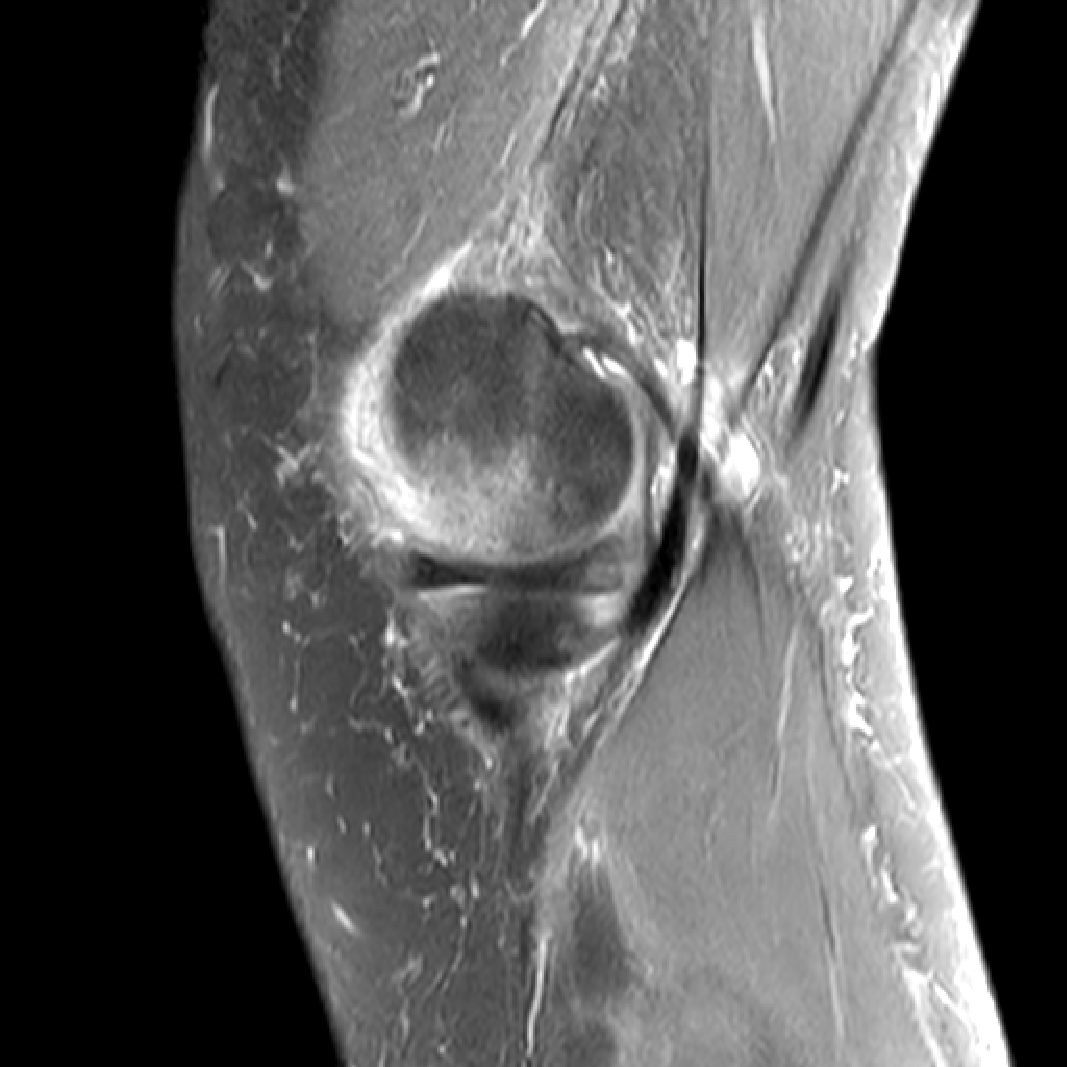
\includegraphics[width=0.85\columnwidth]{corte_rodilla.pdf}
    \caption{Corte sagital de resonancia magnética de rodilla del conjunto RSNA Knee Abnormality Detection\cite{rsnadata}.}
    \label{fig:corte-rodilla}
\end{figure}

Antes de si quiera comenzar con el entrenamiento se verificará la calidad del etiquetado. Una etiqueta ausente no se interpretará automáticamente como ausencia de lesión. de la misma manera, se evaluará la resolución de trabajo mediante inspección visual, en lugar de asumir que una reducción a $64\times64$ conserva toda la información relevante.

\section{Algoritmos y aplicaciones posibles}

Las arquitecturas de esta sección forman parte de la propuesta para los siguientes avances. En esta entrega entrenamos una red completamente conectada sencilla, que se describe en la sección de entrenamiento. Esto nos permite tener un primer punto de comparación antes de comenzar con convoluciones.

\subsection{CNN de referencia}

Como punto de partida proponemos una CNN 2D con tres bloques de convolución, activación ReLU y reducción espacial mediante \textit{max pooling}. Una capa de agrupación global y una capa densa producirán la representación de cada corte. Para obtener una predicción por estudio se combinarán las representaciones de los cortes seleccionados antes de la capa de salida.

Con este modelo podemos comprobar el funcionamiento del procesamiento y establecer una referencia entrenada desde cero. La limitación principal prevista es la dificultad para aprender representaciones robustas cuando las etiquetas supervisadas son escasas. El entrenamiento y, en general, el desempeño de la red también se podrá haber visto afectado por omitir información relevante al momento de escoger ciertos cortes. Por lo que es necesario documentar qué cortes están usando y mantenerse consistente.

\subsection{Aprendizaje por transferencia con ResNet-18}

La alternativa principal sería una ResNet-18 preentrenada, adaptada a imágenes de resonancia. ResNet incorpora conexiones residuales que facilitan el entrenamiento de redes profundas \cite{he2016}. Con esta podemos extraer características de cada corte y agregar estas características por serie y estudio mediante promedio o máximo.

El modelo final tendría doce salidas con activación sigmoide, que deveulva la probabilidad independiente de que cierto estdio tenga tal diagnosticoo. Como ya habíamos mencionado, los diagnósticos pueden coexistir, por lo que no se usará \textit{softmax}. Inicialmente se entrenará la nueva capa de salida y después se evaluará un ajuste de los últimos bloques convolucionales. Aunque es cierto que el beneficio de usar una red ya preentrenada tiene que comprobarse haciendo ciertos experimentos porque sus imágenes originales difieren de las resonancias.

Parte de esta propuesta tiene una mención en MRNet \cite{bien2018}. Nuestro proyecto tomará esa idea como referencia metodológica pero sin brincar a la conclusión de que sus resultados y los nuestros puedan coincidir. Es decir que el desempeño de su red sea igual que el de la nuestra. Esto por el método de entrenamiento, las decisiones que se tomaron para ese estudio en específico y que además no clasifican las mismas etiquetas como tal.

\subsection{Alternativas de eficiencia y contexto espacial}

EfficientNet-B0 puede ser una posible segunda arquitectura preentrenada si los recursos y el tiempo permiten la comparación. Claro que la las selecciones estan sujetas a cambios con base a lo visto en el curso y lo que la capacidad computacional que tengamos al alcance. La familia EfficientNet estudia el balance entre profundidad, anchura y resolución \cite{tan2019}. En este proyecto se evaluaría como extractor de características, comparando desempeñoy eficiencia (memoria y tiempo) en la misma particion de datos.

También podría explorarse una CNN 3D que pordria ser una extensión posterior para procesar volúmenes mas latos pero exige mas memoria y un tratamiento consistente de espacio. Teniendo en cuenta que es la primera vez que experimentamos con redes y al igual por viabilidad, vamos a comenzar con el enfoque 2D y agregación por estudio.

\subsection{Aplicaciones reales y alcance}

Un caso bien documentado de este tipo de clasificación y que se mantuvo en mente desde que se escogió el dataset es MRNet, que estudió el apoyo a la lectura de resonancias de rodilla \cite{bien2018}. A partir de ese estudio planteamos tres aplicaciones futuras. El apoyo de una segunda lectura para señalar hallazgos que requieren revisión, la priorización de estudios potencialmente anormales y la indexación de colecciones para investigación.

Claro que su implementación en casos reales requeriría validación externa, pero también es cierto que un gran porcentaje de los modelos desarrollados en general, se quedan en notebooks y no se les da seguimiento. Creemos firmemente que cada modelo desarrollado debe de tener una aplicación o alguna aportación real. En este caso el propósito de desarrollar el modelo no es hacer una herramienta autorizada para uso clínico ni se afirmará que reduce tiempos o mejora diagnósticos sin evidencia propia. En este caso buscamos aprender cómo desarrollar modelos de redes profundas para, en un futuro, podamos desarrollar otras que lleguen a la fase de producción.


\section{Metodología}

En esta sección se conserva la propuesta de cómo preparar las imágenes y entrenar las arquitecturas convolucionales que ya habíamos mencionado. La intención para los siguientes avances es comparar nuestra CNN de referencia con una ResNet-18 preentrenada, usando los mismos estudios y cortes. Es importante mencionar que estos valores siguen siendo un punto de partida para esa etapa. El primer entrenamiento de esta entrega utiliza una red completamente conectada y una preparación más sencilla, que se documentan en la sección siguiente.

\subsection{Unidad de análisis y supervisión}

La red recibiría varios cortes de un estudio y devolvería doce probabilidades, una por cada hallazgo. Como ya habíamos mencionado, las etiquetas corresponden a todo el estudio. Esto significa que una lesión señalada en el reporte no tiene que aparecer en cada una de las imágenes de esa rodilla.

Al revisar \texttt{train.csv} encontramos 4\,407 estudios, de los cuales 58 tienen etiquetas binarias y 4\,349 cuentan con reportes sin esas etiquetas. Para poder usar estos últimos proponemos buscar términos en los reportes y revisar si una lesión se afirma, se niega o se menciona con duda. Si el texto afirma que está presente, se asignaría 1; si dice explícitamente que no está, se asignaría 0. Si no la menciona o no es claro, se dejaría sin etiqueta.

Con esto podemos obtener lo que se conoce como etiquetas débiles, ya que salen de interpretar el texto del reporte. Aunque es cierto que este proceso puede tener errores, por lo que debemos revisar manualmente una muestra y comprobar que las etiquetas coincidan con lo escrito. Esto no significa que estemos haciendo una nueva evaluación clínica de las imágenes.

En el planteamiento anterior se propuso guardar los 58 estudios etiquetados para una evaluación final. Para este primer ejercicio decidimos utilizarlos en entrenamiento y validación, porque nos permiten trabajar con etiquetas explícitas sin comenzar todavía con la extracción de etiquetas débiles. Esto significa que esos estudios ya no pueden presentarse después como una prueba final independiente. Para la etapa convolucional tendremos que definir una evaluación independiente y ampliar los datos de entrenamiento. La separación debe hacerse por estudio y mantener juntos los casos de un mismo paciente, cuando se pueda identificar, y los reportes idénticos. Con esto buscamos evitar que información repetida aparezca en ambos conjuntos.

Para la etapa posterior, el número de estudios que terminemos usando dependerá de las etiquetas que podamos extraer y de las imágenes disponibles. Si usamos etiquetas débiles en validación, debemos considerar que su desempeño puede verse afectado por errores en esas etiquetas. En el experimento actual, las etiquetas de entrenamiento y validación son las binarias que ya están disponibles.

\subsection{Selección y preprocesamiento de imágenes}

Como punto de partida descargaríamos un subconjunto de estudios completos que podamos manejar con nuestros recursos. El DICOM que ya descargamos sirve para mostrar un corte en el reporte, pero una sola imagen no es suficiente para entrenar la red.

Antes de comenzar con el entrenamiento se propone seguir estos pasos:
\begin{enumerate}
    \item Leer las imágenes DICOM con \texttt{pydicom} y los decodificadores necesarios para archivos comprimidos \cite{pydicompixels}. Si algún archivo está dañado, se excluiría y se dejaría registrado.
    \item Escoger como máximo una serie sagital, una coronal y una axial. Se daría preferencia a las secuencias sensibles al líquido y a las que tengan supresión de grasa. Si hay varias opciones iguales, se escogería por identificador de serie, manteniendo siempre el mismo criterio.
    \item Ordenar los cortes usando su posición y orientación dentro del DICOM. Si estos datos no permiten ordenar una serie, habría que revisar el caso y documentarlo. El nombre del archivo no nos dice en qué parte de la rodilla está el corte.
    \item Tomar hasta 16 cortes repartidos uniformemente a lo largo de cada serie. Si una serie tiene menos, se usarían los disponibles.
    \item Aplicar la transformación de modalidad cuando corresponda y revisar cómo se representan los tonos de gris. Para normalizar las intensidades de cada serie usaríamos los percentiles 1 y 99, sin contar los píxeles de relleno. Los valores quedarían entre $[0,1]$ y las series sin variación útil se revisarían.
    \item Cambiar el tamaño de los cortes a $224\times224$, manteniendo su proporción.
\end{enumerate}

Para usar ResNet-18 repetiríamos la misma imagen en tres canales. Esto se hace porque la red original recibe tres canales, aunque nuestras imágenes sean en escala de grises. No significa que estemos agregando color o información nueva. Después se aplicarían las medias $(0.485,0.456,0.406)$ y desviaciones $(0.229,0.224,0.225)$ asociadas a sus pesos de ImageNet \cite{torchresnet}. Se mantendría toda la imagen, en lugar de recortar automáticamente su parte central.

Nuestra CNN recibiría un solo canal normalizado. También proponemos usar rotaciones pequeñas para aumentar la variedad de las imágenes de entrenamiento. La rotación debe ser consistente entre los cortes de una serie. Para validación y evaluación no se aplicarían estas variaciones.

\subsection{Arquitectura de la CNN de referencia}

Como ya se propuso en la primera entrega, nuestra CNN tendría tres bloques para extraer características de cada corte:
\begin{itemize}
    \item Convolución con 32 filtros de $3\times3$, ReLU y \textit{max pooling} de $2\times2$.
    \item Convolución con 64 filtros de $3\times3$, ReLU y \textit{max pooling} de $2\times2$.
    \item Convolución con 128 filtros de $3\times3$, ReLU y \textit{max pooling} de $2\times2$.
\end{itemize}

Las convoluciones tendrían desplazamiento 1 y relleno 1, mientras que el \textit{pooling} tendría desplazamiento 2. Con esto, el tamaño de los mapas pasaría de 224 a 112, luego a 56 y finalmente a 28. Después se usaría una agrupación promedio global para obtener un vector de 128 características por corte. Es decir, resumiríamos cada mapa de características mediante un promedio.

Primero se calcularía el promedio de los vectores de los cortes válidos de cada serie y después el de las series disponibles. Con esto podemos juntar la información sin darle más peso a una serie solamente porque tiene más imágenes. El vector del estudio pasaría por \textit{dropout} con probabilidad 0.2 y una capa densa de doce salidas. El \textit{dropout} desactiva temporalmente algunas características durante el entrenamiento para reducir la dependencia de la red en unas pocas de ellas.

\subsection{Arquitectura con ResNet-18}

La alternativa principal sería una ResNet-18 con pesos preentrenados en ImageNet. Se quitaría su clasificador original y se conservaría la parte que extrae características, que devuelve un vector de 512 valores por corte \cite{he2016,torchresnet}. Después se juntarían los cortes y las series con el mismo método que en nuestra CNN. También se usaría \textit{dropout} de 0.2 y una capa densa de doce salidas.

Este promedio se puede expresar de la siguiente manera. Para un estudio $i$ con $S_i$ series y $T_{is}$ cortes válidos en la serie $s$:
\begin{equation}
h_i=\frac{1}{S_i}\sum_{s=1}^{S_i}
\left(\frac{1}{T_{is}}\sum_{t=1}^{T_{is}}f_\theta(x_{ist})\right).
\end{equation}
Aquí, $f_\theta$ es la parte de la red que extrae características y $x_{ist}$ representa un corte. La expresión primero promedia los cortes de cada serie y después las series del estudio. Si alguna serie falta, no se tomaría en cuenta. Si un estudio no tiene ninguna serie que podamos usar, se excluiría y se dejaría registrado.

Con una red preentrenada podemos empezar con características visuales que ya fueron aprendidas. Aunque es cierto que todavía debemos comprobar si eso ayuda con las resonancias. Por ahora nos concentraríamos en estos dos modelos, dejando EfficientNet y las redes 3D como posibles extensiones.

\subsection{Funciones de activación}

Dentro de los bloques convolucionales se usaría ReLU:
\begin{equation}
\operatorname{ReLU}(a)=\max(0,a).
\end{equation}
Esta función deja pasar los valores positivos y convierte los negativos en cero. Con ella podemos introducir relaciones no lineales en la red. Para backpropagation, su derivada es 1 cuando el valor es positivo y 0 cuando es negativo. En cero se usaría la convención de derivada 0.

La capa densa devolvería doce valores reales, llamados \textit{logits}, $z_{ik}$. Para convertir el valor del hallazgo $k$ en una probabilidad se usaría sigmoide:
\begin{equation}
p_{ik}=\sigma(z_{ik})=\frac{1}{1+e^{-z_{ik}}}.
\end{equation}
Como ya habíamos mencionado, un estudio puede presentar varios hallazgos al mismo tiempo. Por eso cada salida se calcula por separado y las probabilidades no tienen que sumar 1. Como referencia inicial se usaría un umbral de 0.5 para clasificar, aunque este esta sujeto a cambios. Si después se prueban otros umbrales, se escogerían usando únicamente la validación.

\subsection{Función de pérdida}

La función de pérdida propuesta sería entropía cruzada binaria, porque para cada hallazgo queremos estimar si está presente o ausente. Es importante recordar que no tener una etiqueta no significa que no exista una lesión. Por eso se usaría una máscara $m_{ik}$, que vale 1 cuando tenemos una etiqueta que podemos usar y 0 cuando falta.

Para un lote de $B$ estudios, la pérdida se calcularía así:
\begin{align}
\ell_{ik} &=-y_{ik}\log p_{ik}
            -(1-y_{ik})\log(1-p_{ik}),\\
M &= \sum_{i=1}^{B}\sum_{k=1}^{12}m_{ik},\\
\mathcal{L} &= \frac{1}{M}
\sum_{i=1}^{B}\sum_{k=1}^{12}m_{ik}\ell_{ik}.
\end{align}
Aquí, $y_{ik}$ sería la etiqueta 0 o 1 cuando $m_{ik}=1$. La primera expresión calcula el error para un hallazgo, $M$ cuenta las etiquetas disponibles y la última expresión obtiene el promedio de esos errores. Si un lote no tiene etiquetas que podamos usar, no se actualizarían los pesos con ese lote.

En PyTorch se usaría \texttt{BCEWithLogitsLoss} sin reducción automática. Después se aplicaría la máscara y se dividiría entre $M$. Esta función ya combina sigmoide y entropía cruzada de manera numéricamente estable \cite{torchbce}. Por eso la red le pasaría directamente los \textit{logits}, sin aplicar antes otra sigmoide. La sigmoide se usaría al momento de obtener las probabilidades para evaluar la red.

Como punto de partida se usaría la pérdida sin ponderaciones. Si encontramos que algunas categorías están mucho más representadas que otras, se podrían probar pesos por categoría. Estos se calcularían solamente con los datos de entrenamiento, sin usar las frecuencias del grupo de evaluación.

\subsection{Backpropagation y actualización de pesos}

En cada lote, primero se pasarían las imágenes por la red para obtener sus salidas y calcular la pérdida. Después se usaría backpropagation para calcular cómo contribuyó cada parámetro a ese error. Esto se hace mediante la regla de la cadena, pasando las derivadas desde la salida hacia las capas anteriores. En PyTorch podemos calcular estos gradientes con diferenciación automática \cite{torchautograd}.

Para la pérdida sin ponderaciones que se propuso, el gradiente respecto a cada \textit{logit} sería:
\begin{equation}
\frac{\partial\mathcal{L}}{\partial z_{ik}}
=\frac{m_{ik}}{M}(p_{ik}-y_{ik}).
\end{equation}
Con esta expresión podemos ver que una etiqueta desconocida no aporta gradiente, porque su máscara vale cero. Los gradientes pasan por la capa densa, los promedios y las convoluciones para ajustar los parámetros que estamos entrenando. En \textit{max pooling}, el gradiente pasa a la posición que se escogió como máximo. En el promedio se reparte entre los elementos válidos.

El optimizador propuesto sería Adam, que usa estimaciones de los momentos de los gradientes para ajustar los pesos \cite{torchadam}. Antes de procesar cada lote se limpiarían los gradientes acumulados. Después se calcularían los nuevos con backpropagation y se haría la actualización. Con esto se repite el proceso de obtener una predicción, calcular su error y ajustar la red.

\subsection{Configuración inicial y evaluación}

Nuestra CNN se entrenaría desde cero, con pesos iniciales aleatorios. Para ResNet-18 se entrenaría primero la capa de salida durante cinco épocas, dejando fijos los pesos del extractor y sus estadísticas de normalización. Después se evaluaría ajustar el último bloque residual junto con el clasificador. Una época corresponde a recorrer el conjunto de entrenamiento una vez.

Los valores iniciales que proponemos son:
\begin{itemize}
    \item Lotes de 2 estudios, ajustables según la memoria disponible.
    \item Adam con tasa $10^{-3}$ para nuestra CNN y para el clasificador cuando el extractor de ResNet-18 esté fijo.
    \item Para ajustar ResNet-18: tasa $10^{-4}$ para el último bloque y $10^{-3}$ para el clasificador.
    \item Hasta 20 épocas en total, deteniendo el entrenamiento si pasan cinco épocas sin mejorar la pérdida de validación.
    \item Semilla 42 y registro de la separación de datos, series, cortes, versiones y configuración.
\end{itemize}

Todo sujeto a cambios por limitantes como tiempo o capacidad computacional. Se conservaría el modelo que tenga la menor pérdida de validación. Una vez tomadas las decisiones de entrenamiento, se necesitará un conjunto independiente para la evaluación final. Los 58 estudios ya utilizados en este avance no cumplen esa función. Se reportarían ROC-AUC por hallazgo, el promedio macro de las categorías que se puedan calcular, sensibilidad, precisión y F1. También se indicaría cuántos casos se evaluaron y qué categorías no tienen positivos o negativos.

Aunque es cierto que 58 estudios son pocos para sacar conclusiones generales. Por eso los resultados servirían como una primera evaluación y no como prueba de que la red funciona igual en cualquier población. La intención es aplicar lo visto en funciones de activación y backpropagation a nuestro problema, comprobando primero que podemos obtener etiquetas confiables y trabajar con las imágenes y recursos disponibles.


\section{Entrenamiento: primeros experimentos, curvas de aprendizaje preliminares e hiperparámetros probados}

\subsection{Objetivo de este primer entrenamiento}

En este avance entrenamos una red completamente conectada sencilla. Como ya habíamos mencionado, las redes convolucionales quedan para la siguiente etapa. Por ahora el objetivo es tener un modelo que entrene de verdad y observar cómo cambian sus resultados cuando modificamos la tasa de aprendizaje o el número de neuronas y capas. Este primer modelo nos sirve como una referencia inicial, aunque todavía no tenga un buen desempeño.

Es importante mencionar que aquí no entrenamos la CNN ni ResNet-18 que se propusieron en la metodología. Tampoco utilizamos características obtenidas con una red preentrenada. La red recibe directamente los valores de las imágenes preparadas, y aprende sus pesos desde una inicialización aleatoria.

\subsection{Datos utilizados y preparación de las imágenes}

Utilizamos los 58 estudios que tienen etiquetas explícitas para los doce hallazgos. Para cada estudio escogimos una sola serie sagital, dando preferencia a las secuencias sensibles al líquido y a las que tienen supresión de grasa. Cuando había varias opciones, se resolvió la selección por el identificador de serie. En total descargamos 290 archivos DICOM, que corresponden a cinco cortes por estudio. La descarga fue selectiva y no se descargó el conjunto completo.

Para escoger los cinco archivos ordenamos el listado de cada serie por su UID y tomamos posiciones repartidas en ese listado. Aunque es cierto que esto nos permite repetir la selección, el UID no nos dice en qué parte de la rodilla está el corte. Por eso no podemos afirmar que sean cinco posiciones anatómicas repartidas uniformemente. Después de descargarlos sí ordenamos esos cinco cortes usando su posición y orientación dentro del DICOM. Esta forma de seleccionar archivos es una simplificación del ejercicio y puede dejar fuera imágenes donde aparece una lesión.

Cada corte se leyó con \texttt{pydicom}. Aplicamos la transformación de modalidad cuando correspondía, excluimos los píxeles de relleno y ajustamos sus intensidades con los percentiles 1 y 99. Los valores quedaron entre 0 y 1. También se corrigió la representación de tonos de gris cuando la imagen utilizaba MONOCHROME1. Después cambiamos su tamaño a $32\times32$, manteniendo la proporción mediante relleno.

Escogimos una resolución pequeña para poder comenzar con una red densa y un entrenamiento corto. Claro que reducir tanto una resonancia elimina detalle, por lo que no estamos suponiendo que esta resolución conserve toda la información necesaria. Los cinco cortes se juntaron y aplanaron en un vector de $5\times32\times32=5\,120$ valores por estudio. Cada estudio produce una sola predicción de doce hallazgos; sus cortes no se trataron como pacientes independientes.

\subsection{Separación de entrenamiento y validación}

La separación se hizo con una proporción aproximada de 80\% para entrenamiento y 20\% para validación, usando la semilla 42. Se mantuvieron juntos los casos que compartían identificador de paciente y los que tenían reportes idénticos, después de normalizar mayúsculas y espacios. Los identificadores de paciente estaban disponibles y eran distintos entre los 58 estudios. Los reportes se usaron solamente para revisar duplicados; no se utilizaron como entrada ni para generar nuevas etiquetas.

La partición final quedó en 46 estudios para entrenamiento y 12 para validación. Conservamos esa misma separación para los tres experimentos. También calculamos la media y desviación globales de los píxeles únicamente con entrenamiento y usamos esos valores para normalizar ambos conjuntos. Con esto evitamos utilizar información de validación en ese ajuste.

No se separó un conjunto de prueba adicional, porque el alcance de este ejercicio es exploratorio y los datos son pocos. La validación se utilizó para comparar las configuraciones y escoger la época que conservamos. Por eso sus métricas no deben interpretarse como una evaluación final independiente.

\subsection{Red completamente conectada y entrenamiento}

La primera arquitectura tiene 5\,120 entradas, una capa oculta de 64 neuronas con ReLU y una capa de doce salidas. Para probar una red con más capacidad también utilizamos dos capas ocultas de 128 y 64 neuronas, ambas con ReLU. No se aplicaron convoluciones, \textit{dropout}, aumento de datos ni ponderaciones por categoría en este primer experimento.

Las doce salidas son \textit{logits}. Para entrenar usamos \texttt{BCEWithLogitsLoss}, que combina sigmoide y entropía cruzada binaria de forma numéricamente estable \cite{torchbce}. Como todos los estudios utilizados tienen etiquetas completas, no fue necesario aplicar la máscara de etiquetas faltantes propuesta para la etapa de supervisión débil. La pérdida promedia las doce etiquetas de los estudios de cada lote.

Después de calcular la pérdida, usamos backpropagation con \texttt{loss.backward()} y actualizamos los pesos con Adam \cite{torchautograd,torchadam}. Para evaluar convertimos los \textit{logits} en probabilidades con sigmoide y aplicamos un umbral fijo de 0.5. Como ya habíamos mencionado, un estudio puede presentar varios hallazgos, por lo que no se usó \textit{softmax}.

\subsection{Hiperparámetros probados}

Probamos las tres configuraciones de la Tabla~\ref{tab:ff-config}. Las tres se entrenaron durante 40 épocas con lotes de ocho estudios, usando CPU y dos hilos de PyTorch. Cada ejecución comenzó con pesos nuevos y semilla 42. Mantuvimos las mismas imágenes y partición para que las diferencias se relacionaran con los hiperparámetros probados.

\begin{table}[H]
\centering
\caption{Configuraciones de la red completamente conectada.}
\label{tab:ff-config}
\small
\setlength{\tabcolsep}{4pt}
\begin{tabular}{lccc}
\hline
\textbf{Exp.} & \textbf{Capas ocultas} & \textbf{Tasa} & \textbf{Parámetros}\\
\hline
A & 64 & $10^{-3}$ & 328\,524\\
B & 64 & $10^{-4}$ & 328\,524\\
C & 128, 64 & $10^{-3}$ & 664\,524\\
\hline
\end{tabular}
\end{table}

Entre A y B cambiamos solamente la tasa de aprendizaje. Entre A y C cambiamos la anchura y profundidad de la red. En esta ocasión no variamos el número de épocas, para observar las tres curvas durante el mismo periodo.

Se ejecutaron las 40 épocas completas, sin parada temprana, y guardamos los pesos de la época con menor pérdida de validación. Esto permite observar qué sucede después de ese mínimo sin confundir el modelo conservado con el de la última época. Los tiempos de entrenamiento fueron aproximadamente 2.06, 2.08 y 2.35 segundos para A, B y C, respectivamente. Estos tiempos no incluyen la descarga, preparación de imágenes ni generación de las gráficas, y corresponden únicamente a este conjunto pequeño.

\subsection{Curvas de aprendizaje y resultados}

Al terminar cada época calculamos la pérdida y la exactitud binaria de entrenamiento y validación con los mismos pesos. La exactitud binaria cuenta las etiquetas individuales acertadas entre todas las etiquetas evaluadas. No significa que ese porcentaje de estudios tenga todos sus hallazgos correctos, ni representa una precisión clínica.

Las Figuras~\ref{fig:ff-perdida} y~\ref{fig:ff-exactitud} muestran las curvas obtenidas en los entrenamientos reales. La línea vertical señala la época cuyos pesos se conservaron. Las gráficas usan la misma escala entre configuraciones para facilitar la comparación.

\begin{figure*}[t]
\centering
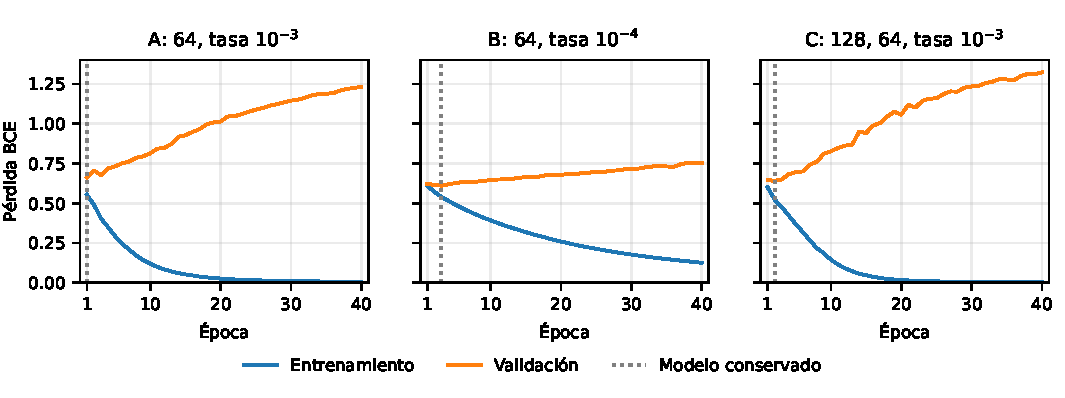
\includegraphics[width=0.98\textwidth]{ff_perdida.pdf}
\caption{Pérdida de entrenamiento y validación durante 40 épocas. La línea punteada marca el modelo conservado por menor pérdida de validación. En los tres experimentos la pérdida de entrenamiento baja mientras la de validación termina aumentando.}
\label{fig:ff-perdida}
\end{figure*}

\begin{figure*}[t]
\centering
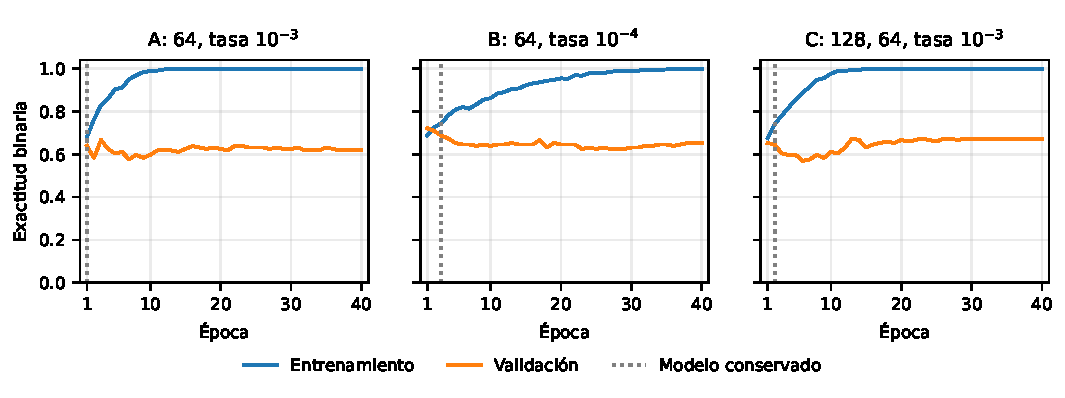
\includegraphics[width=0.98\textwidth]{ff_exactitud.pdf}
\caption{Exactitud binaria de entrenamiento y validación. Al final las tres redes alcanzan 1.0 en entrenamiento, mientras que la validación permanece considerablemente por debajo.}
\label{fig:ff-exactitud}
\end{figure*}

Para tener una referencia adicional calculamos la frecuencia de cada hallazgo en los 46 estudios de entrenamiento. Después usamos esas doce frecuencias como probabilidades constantes para todos los estudios de validación. Esta referencia no aprende de las imágenes, pero nos permite comprobar si la red aporta algo más que predecir de acuerdo con las etiquetas más frecuentes.

La Tabla~\ref{tab:ff-resultados} presenta las métricas de validación de los modelos conservados. El AUC macro se calculó sobre diez hallazgos, porque en validación no hubo positivos de osteoartritis tibiofemoral lateral ni de fractura. Para esas dos categorías no se puede calcular AUC ni sensibilidad. El F1 micro reúne los verdaderos positivos, falsos positivos y falsos negativos de las doce salidas.

\begin{table}[H]
\centering
\caption{Resultados de validación del modelo conservado en cada experimento.}
\label{tab:ff-resultados}
\small
\setlength{\tabcolsep}{5pt}
\begin{tabular}{lcccc}
\hline
\textbf{Exp.} & \textbf{Época} & \textbf{Pérdida} & \textbf{F1 micro} & \textbf{AUC macro}\\
\hline
A & 1 & 0.6634 & 0.3810 & 0.4613\\
B & 3 & 0.6104 & 0.3478 & 0.4627\\
C & 2 & 0.6409 & 0.2609 & 0.4169\\
Constante & -- & 0.5850 & 0.3810 & 0.5000\\
\hline
\end{tabular}
\end{table}

La exactitud binaria de esos mismos modelos fue 0.6389 para A, 0.6875 para B y 0.6458 para C. La referencia constante obtuvo 0.7292. Aunque son valores que parecen más altos que el F1, debemos recordar que acertar etiquetas negativas frecuentes puede aumentar la exactitud sin mejorar la detección de hallazgos positivos.

\subsection{Qué observamos en cada configuración}

En A, la red aprendió rápidamente los estudios de entrenamiento. Su menor pérdida de validación fue 0.6634 en la primera época. Al terminar la época 40, la pérdida de entrenamiento había bajado a 0.0056, pero la de validación había subido a 1.2318. Esto nos muestra que seguir entrenando redujo el error sobre los ejemplos conocidos, sin mejorar los estudios que quedaron fuera del entrenamiento.

En B, al reducir la tasa de aprendizaje a $10^{-4}$, el aprendizaje fue más lento. Su menor pérdida de validación fue 0.6104 en la época 3, la más baja entre las redes probadas. Al final, la pérdida de entrenamiento fue 0.1259 y la de validación 0.7518. El aumento en validación fue menor que en A, aunque también hubo sobreajuste. Claro que tener la menor pérdida no significa ganar en todas las métricas: su F1 micro fue menor que el de A.

En C aumentamos el número de capas y neuronas. La red pasó de 328\,524 a 664\,524 parámetros, pero eso no produjo una mejor generalización de forma consistente. Su menor pérdida de validación fue 0.6409 en la época 2, menor que la de A pero mayor que la de B. Además, su F1 micro y AUC macro fueron menores que los de ambas redes. Al final, la pérdida de entrenamiento fue 0.0026 y la de validación 1.3234. Con esto podemos ver que una red más grande puede aprender muy bien los ejemplos disponibles y aun así fallar al evaluar otros.

Las tres redes alcanzaron una exactitud binaria de 1.0 en entrenamiento al terminar. Sin embargo, la de validación quedó en 0.6181, 0.6528 y 0.6736 para A, B y C en esa última época. La diferencia entre ambos conjuntos, junto con el aumento de la pérdida de validación, es evidencia de sobreajuste en esta partición. El comportamiento es consistente con aprender demasiado los ejemplos de entrenamiento y no generalizar lo suficiente.

\subsection{Limitaciones y aprendizaje de este avance}

La configuración B se escogió por su menor pérdida de validación. Aun así, ninguna de las tres redes superó en pérdida a la referencia constante, que obtuvo 0.5850. Los AUC macro de las redes también quedaron por debajo de 0.5 en esta validación. Por ahora no tenemos evidencia de que la red esté aprovechando las imágenes para mejorar sobre esa referencia.

Aunque es cierto que hay varias limitaciones que pueden influir. Solo usamos 58 estudios, una serie por estudio y cinco cortes reducidos a $32\times32$. La selección de archivos puede omitir lesiones, la reducción elimina detalle y el aplanado no conserva explícitamente las relaciones espaciales que una CNN puede aprovechar. Estos experimentos no permiten determinar por separado cuánto afecta cada decisión.

También debemos considerar que solo hay 12 estudios en validación y que ese mismo conjunto se usó para escoger los modelos. Por eso las métricas pueden cambiar bastante con otros estudios y no representan una prueba independiente. No podemos concluir que la CNN será mejor solamente con estos resultados; tendremos que comprobarlo con una preparación más formal y una comparación que use datos y condiciones compatibles.

Lo que sí logramos fue correr el entrenamiento completo, guardar curvas reales y observar el efecto de cambiar la tasa de aprendizaje y la capacidad de la red. El modelo todavía tiene un desempeño limitado, pero este primer experimento nos permite identificar el sobreajuste y tener una referencia inicial para continuar con el proyecto.

\subsection{Notebook y evidencia del entrenamiento}

El código se organizó en el notebook \texttt{entrega3\_feedforward.ipynb}, con celdas para cargar los datos, separar los estudios, definir la arquitectura, entrenar las tres configuraciones, graficar las curvas y comparar los resultados. Se ejecutaron las nueve celdas de código de principio a fin sin errores y se conservaron sus salidas.

La preparación selectiva de imágenes se encuentra en \texttt{preparar\_ff.py}. También guardamos el manifiesto de archivos y la partición, las historias por época en CSV, los pesos de los modelos conservados, las métricas y las versiones utilizadas. El entorno se administra con UV mediante \texttt{pyproject.toml} y \texttt{uv.lock}. La ejecución registrada usó Python 3.12.14 y PyTorch 2.14.1, con CPU y semilla 42. El notebook y sus resultados acompañan el reporte; los DICOM permanecen en la carpeta local de datos.


\newpage

% quitar comentario para incluir todas las q no estan citadas
% \nocite{*} 
\clearpage
\section{Referencias}
\begingroup
% El encabezado numerado anterior corresponde al punto VII.
% Se evita duplicar el encabezado interno de la bibliografía.
\def\section*#1{}
\insertbibliography{referencias}
\endgroup



%INSERTAR APENDICE SI ES NECESARIO
% \newpage
% \clearpage
% \appendix

% \section*{Anexo A. Nombre de anexo}

% A continuación, se anexa...

% \begin{center}
% \href{url}{\underline{Haga click para redirigirse a ...}}
% \end{center}

\end{document}
